\section{Architettura logica del prodotto} \label{sec:archlogica}

\begin{figure}[h!]
    \centering  
    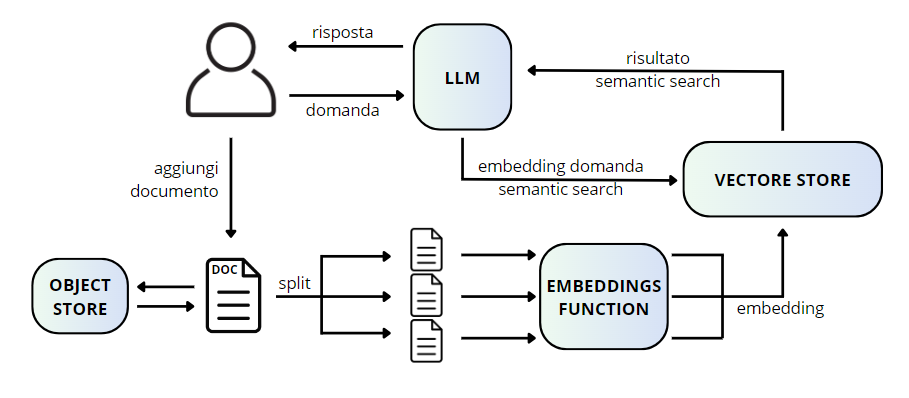
\includegraphics[width=\textwidth]{archlogic.png}
    \caption{Funzionamento del prodotto}
\end{figure}

\noindent Le funzionalità offerte dall’applicazione si suddividono in due categorie: la gestione dei documenti presenti nel sistema, con la possibilità per l’utente di aggiungerne e rimuoverne, e la loro consultazione tramite chatbot.\\
Nella gestione della documentazione presente e utilizzata dal sistema, l’utente può effettuare il caricamento dei documenti dei quali vorrà ricevere le informazioni. I documenti verranno quindi salvati e archiviati tramite MinIO, e successivamente processati. In particolare, ogni documento viene diviso nelle sue singole pagine, e ogni pagina viene suddivisa in chunk, i quali sono successivamente embeddizzati, ovvero elaborati e trasformati in vettori di numeri reali. I valori dello spazio vettoriale generato rappresentano così le parole che compongono i vari documenti. Questo avviene sfruttando funzionalità di embedding date dai large language model utilizzati nel prodotto, ovvero un modello locale di Ollama e GPT-3.5 di OpenAI, e i vettori sono successivamente salvati in modo persistente all’interno del vector store ChromaDB. Qui sono storicizzati in attesa di essere utilizzati in seguito per la formazione delle risposte.\\
Nell’interazione con i documenti presenti nel sistema, l’utente potrà inviare delle domande al chatbot e ricevere risposte riguardanti i documenti caricati in precedenza. Nella formazione e invio della domanda posta dall’utente, il sistema effettua la vettorizzazione della domanda tramite lo stesso processo di embedding utilizzato per i documenti. Per fornire una risposta esatta all’utente, viene effettuata una semantic search sul database vettoriale, andando a comparare la distanza dello spazio vettoriale della domanda, con quello delle informazioni contenute all’interno del vectore store.\\
Una volta completata la semantic search, e identificata la risposta alla domanda posta grazie alla vicinanza del vettore della domanda con quello della risposta, il sistema fornisce il risultato della ricerca semantica al modello large language, che si occuperà della generazione della risposta per l’utente. Nel caso in cui la domanda dell’utente non riguardi i documenti caricati, o più in generale quando non è presente la risposta alla domanda in nessuno dei documenti presenti nel sistema, viene fornita una risposta standard, che informa la non pertinenza della domanda. Questo è possibile grazie a operazioni di prompt engineering nella formulazione della richiesta inoltrata al large language model.\\
Nel caso in cui la risposta alla domanda sia stata identificata in un documento, il chatbot fornisce la risposta, riportando anche il documento che è fonte della risposta data, mostrandone nome e numero della pagina di interesse.\\
Durante la conversazione tra utente e chatbot, i messaggi scambiati sono salvati in modo persistente sul database Postgres, così da poter ricomporre la chat history quando l'utente esce dalla pagina del chatbot. I messaggi vengono eliminati solo quando è l'utente a richiederne l'eliminazione.\\
Oltre a poter inserire nuovi documenti nel sistema, l'utente potrà rimuovere e visionare quelli già presenti e memorizzati su MinIO. Alla rimozione di un documento, sono contestualmente eliminati anche i vettori degli embeddings delle sue pagine. In questo modo, il chatbot non potrà più restituire risposte sul documento non più nel sistema.

\newpage